\section{PermLLM框架}
经过前文的梳理和分析,我们可以看到拆分学习应用于大模型的隐私推断存在严重的隐私泄漏问题,与此同时,密码学方法则存在着严重的计算通讯开销问题。
%
我们注意到,密码学在进行大模型隐私推断时,其主要的开销也在于非线性激活函数GeLU上。
由于GeLU的非线性较强,各种密码学方案往往采用高阶多项式对其进行拟合,从而带来了严重的计算开销。
%
现有研究的分析表明,GeLU、层归一化等的通讯开销甚至可以达到线性计算(矩阵乘法等)的一百多倍。
%
因此,优化基于密码学的大模型隐私推断的关键在于优化非线性函数。
%
%

而上一章提出的基于秘密分享和随机排列的安全神经网络框架正是对神经网络的非线性激活函数进行优化,极大提高了神经网络隐私推断和训练的效率,同时尽可能地维持了安全性。
%
在此基础上,本章我们对此针对大模型进行进一步优化,提出融合密码学方法和随机排列的基础上,实现高效安全的大模型隐私推断框架PermLLM。
%
PermLLM框架面向的场景为两方推断的场景,且存在一个辅助第三方用于离线计算。
%
$P_0$为模型拥有方(如OpenAI),其拥有模型的所有参数信息。
%
$P_1$为用户,其目标是获取大模型的关于自身的文本输入的回复。
%
$P_2$为辅助第三方,其参与离线计算阶段,用于生成安全乘法和安全排列的预计算值。
%
我们采用了半可信的安全性设定,同\autoref{}一致。


我们将大语言模型的计算分为三个部分:线性部分、非线性部分和下标选择阶段。
其中线性阶段包含了线性层、注意力分数计算、层归一化后的逐元素线性映射等;
非线性阶段包含了GeLU激活函数、注意力分数的Softmax计算、层归一化的计算等;
而下标选择阶段则是根据预测的分数安全地产生预测词语的下标的阶段。
%
对于线性阶段,我们通过改进的秘密分享协议进行高效计算;
对于非线性阶段,我们采用基于安全随机排列协议的逐元素计算协议进行计算;
对于下标选择阶段,我们基于随机排列和同态加密设计了安全的下标选择协议,不仅支持常用的选取最大分数的词语,也支持按照概率采样等复杂的下标选择策略。
%


\subsection{隐私推断的三个阶段}
许多基于秘密分享技术的隐私保护机器学习框架会按照两个阶段运行,分别是离线(Offline)阶段和在线(Online)阶段。
%
考虑$P_0$和$P_1$要安全地计算$f(X)$的情况,其中$X$被秘密分享在两方之间,而$f$则是一个固定的函数。
%
在离线阶段,$X$还未出现,$P_0$和$P_1$并不需要知道$X$的具体值。
%
但是其可以对未来的$f(X)$进行一些准备工作,比如生成Beaver三元组来辅助安全乘法计算。
%
在在线阶段,$P_0$和$P_1$得到了$X$的具体值,再进行后续的工作。
%t
通过这种方法,参与方可以在还未进行具体的隐私计算任务时提前准备,从而可以减少具体输入出现后的安全计算的开销。

%
而在PermLLM中,我们采用类似的思想,将隐私推断分为三个阶段,分别是初始化阶段、离线阶段、在线阶段。
%
其中初始化阶段和对应的大模型权重有关,在大模型权重不改变的情况下,初始化阶段仅需执行一次。
%
离线阶段和在线阶段则和一般隐私保护机器学习框架中的定义相同。
每一次离线阶段会产生一些预计算值供在线阶段使用,而每一次在线阶段都会消耗一次离线阶段产生的预计算值。
%
比如,一个可能的运行序列可以是“初始化-离线-在线-离线-在线”,
也可以是“初始化-离线-离线-在线-在线”。
但是“初始化-离线-在线-在线-离线”是一个不合法的顺序,因为第二个在线阶段时已经没有预训练的值供其使用。

\subsection{优化的秘密分享乘法}
一般的秘密分享乘法在每一轮都要针对两个乘数生成对应的Beaver三元组元素$U$和$V$,并且在在线阶段恢复出$X - U$和$Y- V$。
当乘数的尺寸很大时,这种方法会带来巨大的通讯开销。
%
在大语言模型线性层的计算中,乘数的尺寸分别为$d\times d$和$d$,且$d > 10^3$。
以ChatGLM-6B模型为例,$d = 4096$,此时恢复出$X - U$需要传输大约$2\times 4096^2$个浮点数,折合流量$128M$。
%
即普通秘密分享乘法仅仅计算一个线性层就消耗$128M$的流量,导致一次推断中矩阵乘法的总计流量开销超过10Gb,极大降低了大语言模型隐私推断的侠侣。
%
因此,本节考虑到大语言模型推断过程的特性,对秘密分享乘法进行优化。

%

\subsubsection{针对线性层的秘密分享乘法}
我们首先考虑大预言模型中的线性层。
%
线性层的计算可以表示为$W \bvec x + \bvec b$,其中$W \in \mathbb R^{d\times d}$是一个大矩阵,表示权重;$\bvec x \in \mathbb R^{d}$则是输入文本相关的隐层表征。
%
在秘密分享中,共有两次通讯,分别是离线时$P_2$分发Beaver三元组($U\bvec v = \bvec w$)给$P_0$和$P_1$,和在线时$P_0$和$P_1$恢复出$W - U$和$\bvec x - \bvec v$。
%
我们注意到,由于大模型推断过程中权重$W$是固定不变的,我们可以产生一次Beaver三元组中的$U$,同时$W - U$也只需恢复一次。
因此我们可以把这些计算安排到初始化阶段进行。
%
而输入相关的$\bvec x$则会每次变化,因此三元组中的$\bvec v$和对应的$\bvec w=U\bvec v$会被每一次在线运算阶段消耗,需要在每次离线阶段重新生成。
%
因为$W$的大小是$\bvec x$的$d$倍(在大语言模型中$d > 10^3$),因此将有关$W$的计算提前到初始化阶段单次计算,可以极大地减少在线阶段和离线阶段的通讯开销。


我们在\autoref{alg:perm-llm:secure_mul_fixed}中具体描述上述算法。
同时,在\autoref{fig:perm-llm:ssmul}中,我们也对比了原始的秘密分享乘法和优化的$X$固定的秘密分享乘法。
%
利用$X$是$P_0$已知的特性,我们可以把$P_0$计算的$(X-U)(Y-V) + \langle U \rangle_0(Y-V)$,以及$P_1$计算的$\langle U \rangle_1(Y-V)$合并,
变成仅需$P_0$计算$X(Y-V)$。
%
此时$P_1$无需知道$Y-V$,只需将自身的$\langle Y \rangle_1 - \langle V \rangle_1$发送给$P_0$即可。
因此我们进一步将在线阶段的通讯次数从2轮减少到1轮。
%


\begin{algorithm}[h!]
    \caption{$X$为$P_0$拥有的常数的安全乘法\textsf{SecureMul}$_F(X, Y)$}
    \label{alg:perm-llm:secure_mul_fixed}
    \begin{algorithmic}[1]
    \Require $P_0$ 持有常数 $X$. 秘密分享的输入 $\langle Y \rangle$
    
    \Ensure 秘密分享的乘积 $\langle Z \rangle = \langle XY \rangle$
    
    \item[\underline{初始化阶段:}]
    %
    \State $P_2$ 产生随机的 $U$ (和 $X$ 形状相同) 并发送给 $P_0$
    %
    \State $P_0$ 发送 $X - U$ 给 $P_1$
    
    \item[\underline{离线阶段:}]
    \State $P_2$ 产生随机的 $V$ (和$Y$ 形状相同), 并且分享 $V, W \gets UV$ 给 $P_0$ 和 $P_1$
    
    \item[\underline{在线阶段:}]
    \State $P_1$ 发送 $\langle Y \rangle_1 - \langle V \rangle_1$ 给 $P_1$,$P_1$ 恢复 $X - U$
    %
    \State $P_0$ 计算 $\langle Z \rangle_0 \gets X(Y-V) + (X-U)\langle V \rangle_0 + \langle W \rangle_0$
    %
    \State $P_1$ 计算 $\langle Z \rangle_1 \gets (X-U) \langle V \rangle_1 + \langle W \rangle_1$
    \end{algorithmic}
\end{algorithm}


\begin{figure}[h!]
    \centering
    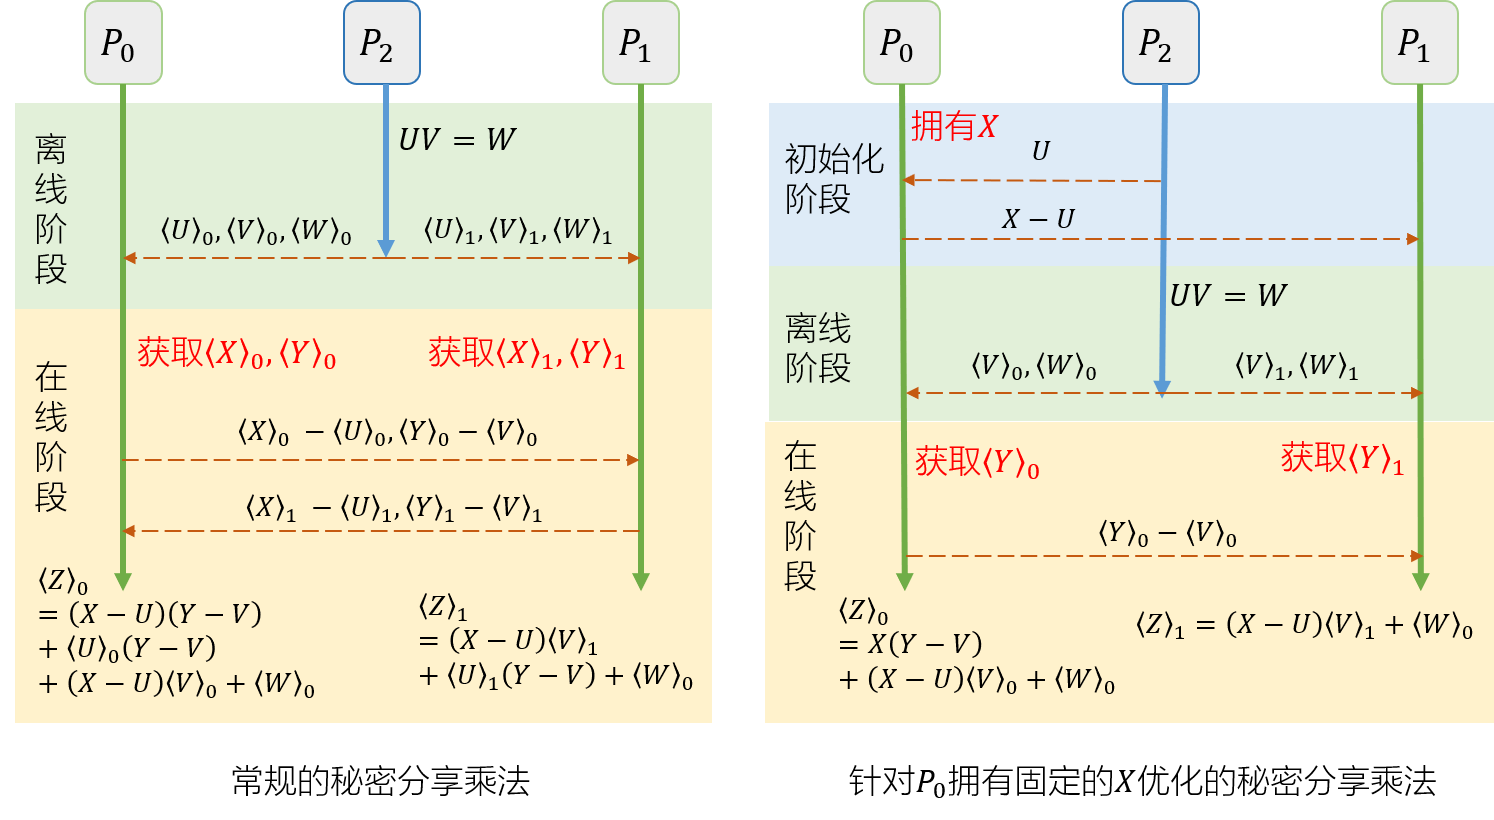
\includegraphics[width=\linewidth]{Z_Resources/perm-llm_ssmul.png}    
    \caption{优化的秘密分享乘法与原始秘密分享乘法的对比}
    \label{fig:perm-llm:ssmul}
\end{figure}
\begin{algorithm}[h]
    \caption{$X$每一轮会拼接的安全乘法\textsf{SecureMul}$_G$}
    \label{alg:perm-llm:secure_mul_growing}
    \begin{algorithmic}[1]
    \Require 分享值 $\langle X' \rangle$, 原有的 $\langle X \rangle$ 以及 $\langle Y \rangle$。
    每一次在线执行时, $X$ 会拼接上 $X'$,即:$X \gets \mathsf{concat}(X, X')$
    
    \Ensure 秘密分享的乘积 $\langle Z \rangle =\langle XY \rangle$
    
    \item[\underline{初始化:}]
    \State 
        $P_0$ 设置 $X - U \gets null, \langle U \rangle_0 \gets null$
        $P_1$ 设置 $X - U \gets null, \langle U \rangle_1 \gets null$
    %
    \State $P_2$ 设置 $U \gets null$.
    
    
    \item[\underline{离线阶段:}]
    \LineComment{我们默认 $\mathsf{concat}(null, U) = U$}
    \State $P_2$ 随机生成 $U', V$ (形状与 $X', Y$一致), 并设置 $U\gets \mathsf{concat}(U, U'), W \gets UV$
    
    \State $P_2$ 分享 $U', V, W$ 给 $P_0$ 和 $P_1$
    
    \item[\underline{在线阶段:}]
    \State $P_0$ 和 $P_1$ 恢复 $X' - U'$ 和 $Y - V$.
    %
    \State $P_0$ 和 $P_1$ 计算 $X - U \gets \mathsf{concat}(X - U, X'-U')$.
    
    \State 
        $P_0$ 计算 $\langle U \rangle_0 \gets \mathsf{concat}(\langle U \rangle_0, \langle U' \rangle_0$).
        $P_1$ 计算 $\langle U \rangle_1 \gets \mathsf{concat}(\langle U \rangle_1, \langle U' \rangle_1$).
    %
    \State $P_0$ 计算 $\langle Z \rangle_0 \gets (X-U)(Y-V) + (X-U)\langle V \rangle_0 + \langle U\rangle_0(Y-V) + \langle W \rangle_0$.
    %
    \State $P_1$ 计算 $\langle Z \rangle_1 \gets (X-U) \langle V \rangle_1 + \langle U\rangle_1(Y-V) + \langle W \rangle_1$.
    \end{algorithmic}
    \end{algorithm}

\subsubsection{针对注意力的秘密分享乘法}
在计算注意力分数时,我们需要将当前的查询向量 $\bvec q_i$ 与多个键向量 $\bvec k_1, \cdots, k_n$ 求内积,且注意到在单次文本生成任务中,每轮都会有一个新的键向量加入。
%
如果把键向量构成的矩阵当作$X$,我们可以发现情况与线性层有所类似。
乘数$X$虽然不是固定的,但是其每一轮只会加入一个新的向量,而其余部分保持不变。
%
因此,我们可以借用针对线性层优化的安全秘密分享乘法中的思想,在每一轮在线阶段的运算中,只考虑 $X$ 新增加的部分(此处记作$X'$)恢复出 $X' - U'$,从而更新原有的 $X - U$上。
%
我们在\autoref{alg:perm-llm:secure_mul_growing}中对算法进行具体描述。


    %

在计算注意力机制时,$X$对应键向量矩阵,第$i$行是$\bvec k_i$。
$X' = \bvec k_n$对应的是根据当前用户输入的最后一个词语新计算的键向量。
%
$Y$对应的就是查询向量 $\bvec q$。
%
可以看出,在每轮交换$X' - U'$而非$X - U$的情况下,在线的通讯开销可以从$nd + d + n$减小为$d + d + n$。
%
由于$d > 10^3$,减少的幅度可以高达$99\%$。

同时,在计算注意力机制的加权和$V^TK \bvec q$时(此时$V^T = [\bvec v_1, \cdots, \bvec v_n]$),$V$每一轮也会拼接上新的值向量,因此我们同样可以采用上述优化的秘密分享矩阵乘法。


\subsection{基于随机排列的非线性函数计算}
现有的基于密码学的大模型隐私推断框架的性能瓶颈主要在非线性激活函数,本节基于\autoref{chap:ss-perm}提出的基于随机排列的非线性函数计算协议,对其进行改进,实现了在线阶段仅需两方参与的非线性函数计算协议。
%

为此,对于一个秘密分享的输入向量$\langle \bvec x \rangle$,我们首先让$P_0$产生一个随机排列$\pi$,然后通过安全的排列协议,在$P_1$上恢复出$\pi[\bvec x]$。
对于逐元素非线性函数$f$,$P_1$计算出$\pi[f(\bvec x)] = f(\pi[\bvec x])$,然后将其分享得到$\langle \pi[f(x)] \rangle$。
%
然后$P_0$和$P_1$再次使用逆排列$\pi^{-1}$执行安全排列协议获得$f(\bvec x)$。
%
此处我们选择\cite{}所提供的秘密分享的安全排列协议。
由于其原始协议是两方的,因此我们可以将其离线计算阶段交给$P_2$执行以提高效率,保留其在线阶段的执行。
%
我们在\autoref{alg:secure_perm}中描述该安全排列协议。
整体的非线性函数计算协议在\autoref{alg:perm-llm:nonlinear}中描述。

\begin{algorithm}[H]
    \caption{安全排列协议\textsf{SecurePerm}}
    \label{alg:secure_perm}
    \begin{algorithmic}[1]
    \Require $P_0$ 持有一个排列 $\pi$. 秘密分享的向量 $\langle \bvec x \rangle$.
    \Ensure 排列后的秘密分享向量 $\langle \bvec y \rangle  = \langle \pi[\bvec x] \rangle$.
    \item[\underline{离线阶段:}]
    \State $P_0$ 发送 $\pi$ 给 $P_2$
    \State $P_2$ 产生随机向量 $\bvec r_1, \bvec r_2 \stackrel{\$}{\gets} \mathbb Z_N $, 并计算 $\Delta \gets \pi[\bvec r_0] - \bvec r_1$
    \State $P_2$ 发送 $\Delta$ 给 $P_0$, 发送 $\bvec r_0, \bvec r_1$ 给 $P_1$
    \item[\underline{在线阶段:}]
    \State $P_1$ 发送 $\langle x \rangle_1 - \bvec r_0$ 给 $P_0$, 并计算 $\langle y \rangle_1 \gets \bvec r_1$
    \State $P_0$ 计算 $\langle y \rangle_1 \gets \pi[\langle x \rangle_0] + \pi[\langle x \rangle_1 - \bvec r_0] + \Delta$
    \end{algorithmic}
\end{algorithm}

\begin{algorithm}[h]
\caption{安全非线性计算\textsf{SecureNonlinear}}
\label{alg:perm-llm:nonlinear}
\begin{algorithmic}[1]
\Require  
    秘密分享的输入 $\langle \bvec x \rangle$,
    一个公开的非线性函数 $f$ 满足 $f(\pi[\mathbf x]) = \pi[f(\mathbf x)]$ 对于某一类随机排列 $\pi$ 都成立
\Ensure 秘密分享的输出 $\langle \mathbf y \rangle = \langle f(\mathbf x) \rangle$
\State $P_0$ 产生一个随机排列 $\pi$
\State $P_0$ 和 $P_1$ 执行 $\langle \pi[\mathbf x] \rangle \gets \mathsf{SecurePerm}(\pi, \mathbf x)$, 然后恢复出 $\pi[\mathbf x]$ on $P_1$
\State $P_1$ 计算 $\langle \mathbf y' \rangle_1 \gets f(\pi[\mathbf x])$,$P_0$ 设置 $\langle \mathbf y' \rangle \gets \mathbf 0$
\State $P_0$ 和 $P_1$ 执行 $\langle \mathbf y \rangle \gets \mathsf{SecurePerm}(\pi^{-1}, \langle \mathbf y' \rangle)$
\end{algorithmic}
\end{algorithm}

注意到,对于一批向量,且必需要进行向量内部的随机排列的场景(如Softmax、层归一化模块),我们可以首先对向量内部元素进行随机排列,然后再对向量顺序进行随机排列。
%
在逆排列时,先对向量顺序进行恢复,再对向量内部元素进行恢复。
%

\subsection{基于同态加密的下标抽取}
当大语言模型计算出最后一层隐层表征后,最后一行向量被用于和输出词向量计算内积,得到预测的下一个词语的可能性分数。
%
有很多方法可以根据分数解码(Decoding)预测的下一个词语,最简单的方法贪心生成算法(Greedy Generation),即选择分数最大的词语,这会使得大语言模型的推断呈现出确定性。
%
如果要使得大语言模型的输出有一定的随机性或多样性,可以按照根据分数使用Softmax等方法算出各个词语的采样概率再进行采样。
%
目前的基于密码学的大模型隐私推断框架,只能支持贪心生成,采用特定密码学协议来计算最大分数的下标(也就是argmax函数)。
%

如果我们直接把分数在$P_1$(用户)上恢复出来,则会导致隐私泄露。
%
这是因为预测分数$\bvec s = W\bvec h$是词向量矩阵与隐层表征的乘积,当$P_1$积累了多个预测分数后,就可以得到
\begin{equation}
    S = (\bvec s_1, \cdots, \bvec s_n) = (W\bvec h_1, \cdots, W\bvec h_n)= WH = \begin{bmatrix}
        \bvec w_1^T H \\ \cdots \\ \bvec w_N^T H,
    \end{bmatrix}
\end{equation}
其中,$n$表示预测分数向量的数量,$N$表示词汇表大小。
可见$S$中的每一行都是经过线性变换$H$后的词向量。
%
虽然从线性变换后的词向量难以还原出原始的词向量,但是其很可能保留了原始词向量的功能,依然可以用来辅助其他语言模型的训练。
由于词向量在语言模型中的地位十分重要,因此我们认为大语言模型的隐私推断必须保护词向量矩阵不被泄露。
%

为了解决这个问题,我们同样采用随机排列的方法。
%
通过随机排列协议,我们可以让$P_1$得到随机排列的分数$\pi[\bvec s]$,然后通过一定的策略产生排列后的下个词语下标$\pi[i]$。
%
此时,$P_1$再和$P_0$执行隐匿查询协议,将$\pi[i]$还原为实际的下标$i$。
%w
我们采用BFV同态加密算法来实现上述隐匿查询协议。
%
BFV是一种同态加密算法,其明文空间为4096维的整数向量(以多项式形式表示),支持密文和明文的向量点积。
%
为此,我们让$P_1$持有同态加密的私钥,然后加密$i$对应的独热向量并发送给$P_0$:

\begin{equation}
    \llbracket \bvec p \rrbracket = \mathsf{Encrypt}[\bvec p], \quad \bvec p = (p_1, \cdots, p_N) \text{ 满足 } p_i = 1, p_{j\ne i} = 0.
\end{equation}
%
$P_1$然后可以执行同态的密文-明文内积运算,求出
\begin{equation}
    \llbracket i \rrbracket = \llbracket \bvec p \rrbracket \odot (\pi^{-1}[1], \cdots, \pi^{-1}[n])
\end{equation}
并发送给$P_0$解密,此时$P_0$得到实际的预测下标$i = \mathsf{Decrypt}[\llbracket i \rrbracket]$。
%
在此过程中,$P_0$只能接触到加密的下标,而$P_1$只能接触到随机排列后的分数。
%
由于每次采用不同的随机排列,因此$P_1$也无法从分数中获取词向量的信息。
%
额外地,由于词汇表大小$N$(词语总数)大于单个密文所能装载的整数数目(4096),我们需要把明文的独热编码和逆排列向量拆分成$L = 4096$大小的片,然后分别内积,最后相加得到最终结果:
\begin{equation}
    \llbracket i \rrbracket = \sum_{j=1}^{N/L} \bvec \llbracket p[jL:(j+1)L] \rrbracket \odot (\pi^{-1}[jL], \cdots, \pi^{-1}[jL + l - 1]),
\end{equation}
其中的求和也是同态求和。
%
我们把上述算法步骤在\autoref{alg:perm-llm:prediction}中正式描述。

\begin{algorithm}[h]
    \caption{安全预测\textsf{SecurePrediction}}
    \label{alg:perm-llm:prediction}
    \begin{algorithmic}[1]
    \Require 秘密分享的分数向量 $\langle \mathbf s \rangle$,$P_1$拥有解码策略$D$
    \Ensure $P_0$ 获得预测的下标 $i = \mathop{\text{argmax}}_i \mathbf s[i]$
    %
    \State $P_0$ 和 $P_1$ 执行安全排列协议: $\langle \pi[\mathbf s] \rangle \gets \mathsf{SecurePerm}(\pi, \langle \mathbf s \rangle)$,然后恢复 $\pi[\mathbf s]$ 给 $P_1$
    \LineComment{只有$P_0$ 知道 $\pi$}
    %
    \State $P_1$ 解码出排列后的下标 $\pi[i] \gets D(\pi[\mathbf s])$
    %
    \State $P_1$ 计算 $\mathbf p \gets \mathsf{onehot}(\pi[i])$, 然后把 $\mathbf p$ 切分成 $\lceil N/L \rceil$ 个长度为 $L$ 的子向量, 即 $\mathbf p_1, \cdots, \mathbf p_{\lceil N/L \rceil}$
    %
    \State $P_1$ 加密得到 $\llbracket p_j \rrbracket \gets \mathsf{Enc}(\mathbf p_j), j  = 1..{\lceil N/L \rceil}$, 然后发送给 $P_0$
    %
    \State $P_0$ 将向量 $(\pi^{-1}[1], \cdots, \pi^{-1}[N])$ 切分成 $\lceil N/L \rceil$ 份 $\mathbf q_1, \cdots, \mathbf q_{\lceil N/L \rceil}$, 然后执行同态的向量内积运算 $\llbracket i \rrbracket \gets (\llbracket \mathbf p_1 \rrbracket \odot \mathbf q_1) \oplus \cdots \oplus (\llbracket \mathbf p_{\lceil N/L \rceil} \rrbracket \odot \mathbf q_{\lceil N/L \rceil})$
    %
    $P_0$发送 $\llbracket i \rrbracket$ 给 $P_1$
    %
    \State $P_1$ 解密得到 $i \gets \mathsf{Dec}(\llbracket i \rrbracket)$
\end{algorithmic}
\end{algorithm}


\subsection{对PermLLM进行优化}
通过上述的三个协议,我们已经可以实现整个大语言模型。
%
具体而言,所有的矩阵(向量、张量)乘法运算可以由秘密共享的乘法实现,而线性层的偏置项可以由$P_0$(模型拥有方)本地加入自身的分享值;而所有的非线性函数,包括GeLU、Softmax, 层归一化(Layer Normalization)都由基于随机排列的非线性计算协议实现;获得了模型产生的分数向量后,再交给安全预测协议产生解码后的单词下标。
%
本节,我们对PermLLM的具体实现提出一些优化,包括将一些参数公开来减少秘密分享乘法的次数,以及采用浮点数秘密分享来提高运算效率。
%
\subsubsection{公开部分参数}
当秘密分享的数乘以一个公开的数时,只需各方将自己本地的分享乘以该数即可:
\begin{equation}
    z = xy \Leftrightarrow \langle z \rangle_i = \langle x \rangle_i y.
\end{equation}
%
因此,我们可以在大语言模型中选取一部分不敏感的参数进行公开,从而减少秘密分享乘法的数目,降低通讯开销。
%
我们选取层归一化模块之后的逐元素乘法(Element-Wise Affine)的权重作为公开的参数。
%
这些权重的参数量(元素个数)在全体参数中的占比低于$0.01\%$,因此几乎可以忽略不记。
但是在不公开的情况下,进行秘密分享的矩阵乘法,则依然会带来通讯伦次,因此在高延迟的网络场景下会带来明显的性能损失。
%
同时,我们也公开位置嵌入的权重,因为这些权重的计算方法往往是公开的,因此无需对其进行隐私保护。
%
我们认为其他的参数是比较重要的,它们不仅参数量占比较大,还和模型的特定功能关系较大。
%
例如,词向量可以用来微调其他的语言模型;而注意力机制中的线性层权重也包含了模型的一些特性,对其进行低秩扰动(LoRA)就可以让大语言模型产生不同特色和功能的文本~\cite{}。
%
在实际情况中,也可以选择更多的公开参数,实现隐私保护和性能之间的权衡。

%
\subsubsection{浮点数秘密分享}
秘密分享起初是在有限域(Finite Domain)上定义的,比如整数环$\mathbb Z_N$。
在这种情况下,秘密分享可以实现信息论的安全,因为任何一方在协议执行过程中接收到的信息都是均匀分布在有限域上的。
%
但是当前的GPU主要面向浮点数的运算,整数运算的效率较低。
因此也有一些工作探究了在浮点数上进行秘密分享~\cite{}。
因此我们可以将(加法)秘密分享推广到浮点数上以提高大语言模型隐私推断的效率。
%
在这种情况下,我们定义秘密分享的分享过程为$x = \langle x \rangle_0 + \langle x \rangle_1$,其中 $\langle x \rangle_0 \sim \mathcal D$。
%
$\mathcal D$ 为一个$\mathbb R$上的随机分布,其规模需要比$x$大很多,从而实现对$x$的充分隐藏。
%
我们假设$x \sim \mathcal X$,则可以让 $\text{Var}[\mathcal D] = \lambda^2 \text{Var}[\mathcal X]$,其中$\lambda$ 控制随机分布的大小,越大的$\lambda$ 可以越好地隐藏$x$。
%
类似地,用于计算乘法$XY=Z$的Beaver三元组也需要按照同样的分布生成:
\begin{equation}
\begin{cases}
    \text{Var}[\langle U \rangle_0] = \text{Var}[\langle U \rangle_1] = \lambda^2 \text{Var}[X], \\
    \text{Var}[\langle V \rangle_0] = \text{Var}[\langle V \rangle_1] = \lambda^2 \text{Var}[Y], \\
    \text{Var}[\langle W \rangle_0] = \lambda^2 \text{Var}[Z].
\end{cases}
\end{equation}
%

在这种情况下,我们可以保证在秘密分享的计算过程中暴露的值都是原始值加上一个很大的噪声,因此可以几乎与原始值无关。
%
但是在某些情况下,如同样的值被多次重复分享,则攻击者可以通过求平均来恢复原始值,从而带来隐私泄漏风险。
%
注意到,浮点数秘密分享对于PermLLM来说并不是必需的,其目的仅在于提高GPU计算的适配性和效率,可以简单地将其更改为整数秘密分享。
%

